\todo{CS4002}
\todo[color=blue!40]{CS4003}
\todo[color=green!40]{CS4004}

En la literatura se han desarrollado diversos métodos para el reensamblaje de objetos 3D rígidos. A continuación, se describen las características de las propuestas más recientes para resolver este problema. \\

El trabajo de Li \textit{et al.} proponen un método de reensamblaje de fragmentos gruesos utilizando los bordes de las caras fracturadas para la correspondencia, y parches cóncavo convexos para la alineación. Este método es eficiente debido a que trabaja sobre las curvas de las caras fracturadas y los parches cóncavo convexos en lugar de todos los puntos del fragmento \cite{3}. Sin embargo, si todos los fragmentos de un objeto no están disponibles, el método falla en la etapa de correspondencia. \\

La investigación de Liao \textit{et al.} introducen un nuevo descriptor (ESPR) invariante a las transformaciones rígidas para la correspondencia, y un árbol de regiones balanceado para la alineación. Este método es eficiente y robusto frente a las transformaciones rígidas en objetos 3D debido a la agrupación y al descriptor propuesto \cite{5}. Sin embargo, la alineación provoca \textit{overlapping}, a causa de que el método solo se enfoca en reducir la distancia entre los fragmentos. \\

La propuesta de Jia \textit{et al.} basan la correspondencia en la similitud de los descriptores de covarianza, y la alineación en el mapeo entre puntos y eliminación de errores. Este método es robusto, debido a que obtiene más del 70\% de \textit{accuracy} con 50\% de ruido, a comparación de otros métodos que obtienen 30\% en promedio \cite{6}. Sin embargo, la experimentación se realizó únicamente sobre \textit{Puzzles 3D}, por lo cual no tenemos resultados sobre el \textit{accuracy} con fragmentos reales. \\

En el método de Wang \textit{et al.}, la correspondencia se realiza con el descriptor LCD, y con la correspondencia potencial se calcula el descriptor SDD para eliminar los pares incorrectos en la etapa de alineación. Este método es versátil porque obtiene resultados notables con fragmentos de diferentes características \cite{7}. Sin embargo, en los casos extremos, como el reensamblaje de objetos con alta curvatura, el \textit{accuracy} disminuye significativamente.

\hfill \break

Por otro lado, los problemas de correspondencia y alineación también han sido explorados de manera independiente. En consecuencia, se han propuesto diferentes enfoques para solucionarlos. No obstante, su exploración dentro del problema reensamblaje aún es limitada. En las siguientes secciones se presentan los trabajos más relevantes de correspondencia y alienación de objetos 3D en los últimos años.

\section{Correspondencia}
El problema de correspondencia de modelos 3D ha sido ampliamente estudiado. Los métodos actuales se pueden dividir en dos categorías: los métodos basados en similitud geométrica y los métodos basados en aprendizaje \cite{18}. \\

Los métodos basados en similitud calculan los descriptores geométricos para los puntos de los modelos 3D, y minimizan la función de energía para encontrar un mapa de correspondencia. Por ejemplo, la propuesta de Ezuz \textit{et al.} minimizan la función de Dirichlet para maximizar la reversibilidad del mapa \cite{f5}. Además, Küpçü y Yemez introducen un método iterativo que minimiza la distancia entre los histogramas de difusión de cada punto \cite{f6}. \\

Los métodos basados en aprendizaje tienen dos vertientes. La primera potencia el \textit{performance} de los métodos basados en similitud geométrica, y la segunda construye los métodos exclusivamente bajo las técnicas de \textit{deep learning} \cite{18}. Por ejemplo, Li \textit{et al.} plantean una arquitectura llamada \textit{Anisotropic Chebyshev spectral CNNs} (ACSCNNs) basada en CNNs y operadores convolucionales sobre los descriptores geométricos \cite{f3}. Mientras que Li \textit{et al.} proponen la red neuronal TC-NET para aprender los descriptores de los puntos \cite{f4}.

\section{Alineación}
El problema de alineación entre escenas 3D ha sido largamente estudiado. Los métodos actuales se pueden dividir en tres categorías: los métodos basados en optimización, los métodos basados en aprendizaje de características y los métodos basados en aprendizaje de transformaciones \cite{9}. \\

Los métodos basados en optimización desarrollan una estrategia sofisticada e iterativa para encontrar la solución óptima al problema no lineal de la ecuación \ref{eq:4} \cite{9}. Por ejemplo, Yuan \textit{et al.} proponen \textit{DeepGMR} para aprender la relación entre los componentes de GMM (modelo de mixturas gausianas) y los puntos del modelo, con la cual se estima los parámetros de transformación con la maximización del \textit{likelihood} en GMM \cite{f7}. \\

Los métodos basados en aprendizaje de características encuentran la transformación a través de la estimación del emparejamiento inicial con \textit{deep learning} y un único paso de optimización (SVD o RANSAC) \cite{9}. Por ejemplo, el método de Wang y Solomon consta de tres etapas para extraer la transformación. La primera extrae los vectores característicos (\textit{Pointnet} o DGCNN), la segunda aproxima la correspondencia entre ellos, y la tercera optimiza con SVD \cite{16}. \\

Los métodos basados en aprendizaje de transformaciones obtienen la matriz de transformación de dos modelos 3D iniciales, para lo cual se considera a la alineación como un problema de regresión o como un \textit{framework} de optimización \cite{9}. Por ejemplo, Choy \textit{et al.} introducen el \textit{framework} de \textit{deep global registration} (DGR), el cual está compuesto por los módulos de extracción y predicción, de análisis de distribución balanceado y de optimización final \cite{10}.

\hfill \break

En este capítulo, se describieron las propuestas más relevantes de los últimos años para resolver los problemas de reensamblaje, correspondencia y alineación en objetos 3D.

\begin{comment}
\section{Parches cóncavo-convexos}

El trabajo de Li \textit{et al.} proponen un método de reensamblaje de fragmentos gruesos utilizando los bordes de las caras fracturadas para la correspondencia, y parches cóncavo convexos para la alineación. \\

La etapa de correspondencia consiste en emparejar fragmentos por medio de la semejanza entre los bordes de las caras fracturadas. Los bordes se extraen con el algoritmo de \textit{boundary tracking} a partir de los puntos con mayor curvatura en el fragmento. Para obtener la semejanza entre $X$ y $Y$ se calculó la distancia euclidiana entre $x_{i} \in X$ y $y_{j} \in Y$ en la vecindad de dos puntos, como se muestra en la ecuación \ref{eq:10} \cite{3}. 

%. Se considera a dos fragmentos emparejados si comparten una curva de al menos $1/8$ de los puntos de la curva más pequeña

\begin{equation} \label{eq:10}
    \Lambda_{i, j} = \frac{1}{3} \sum_{q=-1}^{1} ||x_{i+q} - y_{j+q}||
\end{equation}

La etapa de alineación consiste en tres pasos. Primero, los fragmentos se alinean globalmente a través de los bordes. Segundo, una modificación de \textit{iterative closest point} (ICP) para parches cóncavo convexos refina el alineamiento. Tercero, se aplica una estrategia de validez que verifica la superposición entre las curvas y los parches de los fragmentos \cite{3}. \\

Este método es eficiente debido a que trabaja sobre las curvas de las caras fracturadas y los parches cóncavo convexos en lugar de todos los puntos del fragmento. Sin embargo, si todos los fragmentos de un objeto no están disponibles, el método falla en la etapa de correspondencia.

\section{Árbol balanceado de regiones}

La investigación de Liao \textit{et al.} introducen un nuevo descriptor invariante a las transformaciones rígidas para la correspondencia y un árbol de regiones balanceado para la alineación. \\

La etapa de correspondencia tiene dos pasos principales. Primero, se agrupa el fragmento por regiones con \textit{k-means} para construir el árbol balanceado y reducir el ruido. Segundo, se extiende el descriptor \textit{surflet-pair-relation} (SPR) para que trabaje con regiones y se filtran los pares de fragmentos con mayor cantidad de regiones emparejadas \cite{5}. \\

La etapa de alineación consiste en encontrar los pares de regiones con mayor contacto en el nivel más profundo del árbol. A partir de esta relación inicial, se utiliza ICP sobre los puntos de las regiones encontradas para refinar la alineación entre fragmentos \cite{5}. \\

Este método es eficiente y robusto frente a las transformaciones rígidas en objetos 3D debido a la agrupación y al descriptor propuesto. Sin embargo, la alineación provoca \textit{overlapping}, a causa de que el método solo se enfoca en reducir la distancia entre los fragmentos.

\section{Descriptores de covarianza}

La propuesta de Jia \textit{et al.} basan la correspondencia en la similitud de los descriptores de covarianza, y la alineación en el mapeo entre puntos y eliminación de errores, como se muestra en la imagen.\\

La etapa de correspondencia compara los vectores característicos de los fragmentos $X$ y $Y$ para determinar la semejanza entre ellos. Para este fin, describe las características superficiales locales con la covarianza multiescala entre los \textit{key points} \cite{6}. \\

La etapa de alineación consta de dos pasos principales. Primero, se utilizan los vectores característicos para realizar una alineación global, y se establece un mapeo entre los puntos. Segundo, se eliminan los emparejamientos erróneos del mapeo anterior con \textit{random sample consensus} (RANSAC) \cite{6}. \\



\begin{figure}[!h]
    \centering
    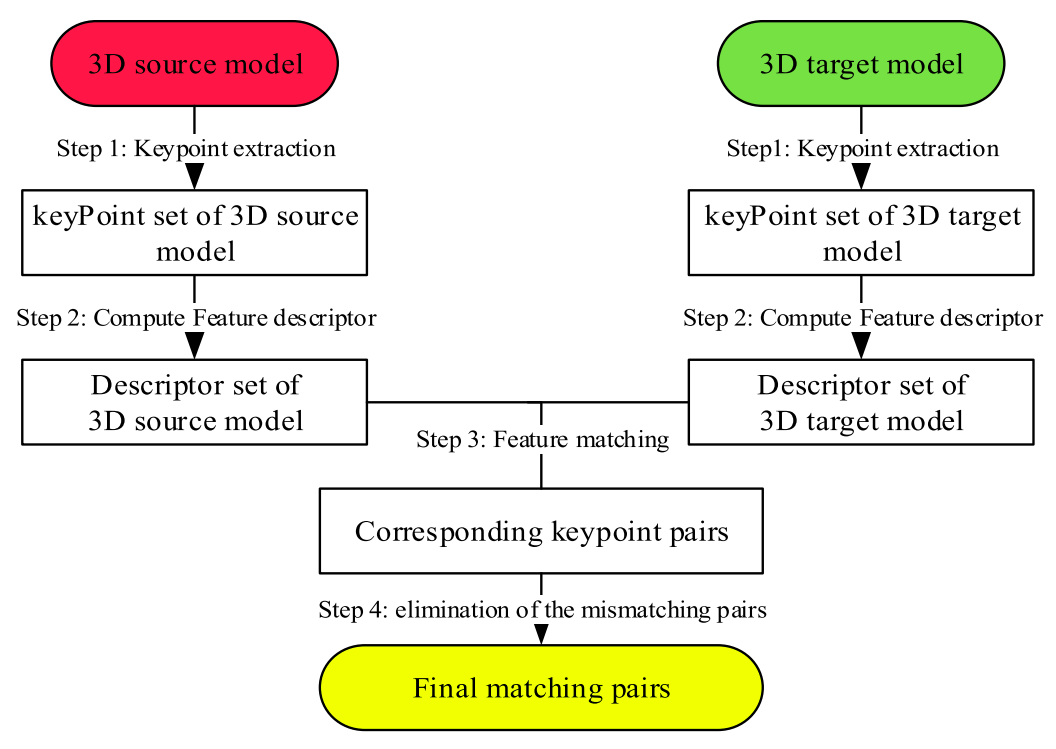
\includegraphics[scale=0.2]{images/covariance.png}
    \caption{\textit{Pipeline} de DGR}
    \label{fig:covariance}
\end{figure}

El método consiste en repetir el emparejamiento por pares hasta que el objeto esté reconstruido. El emparejamiento tiene cuatro pasos principales como se muestra en la figura \ref{fig:covariance}. En el primero, se extrae los \textit{key points}. En el segundo, se calcula la covarianza multiescala para describir las características superficiales locales. En el tercero, se realiza la correspondencia entre los vectores característicos. Y en el cuarto, se eliminan las correspondencias falsas con RANSAC \cite{6}.

\begin{figure}[!h]
    \centering
    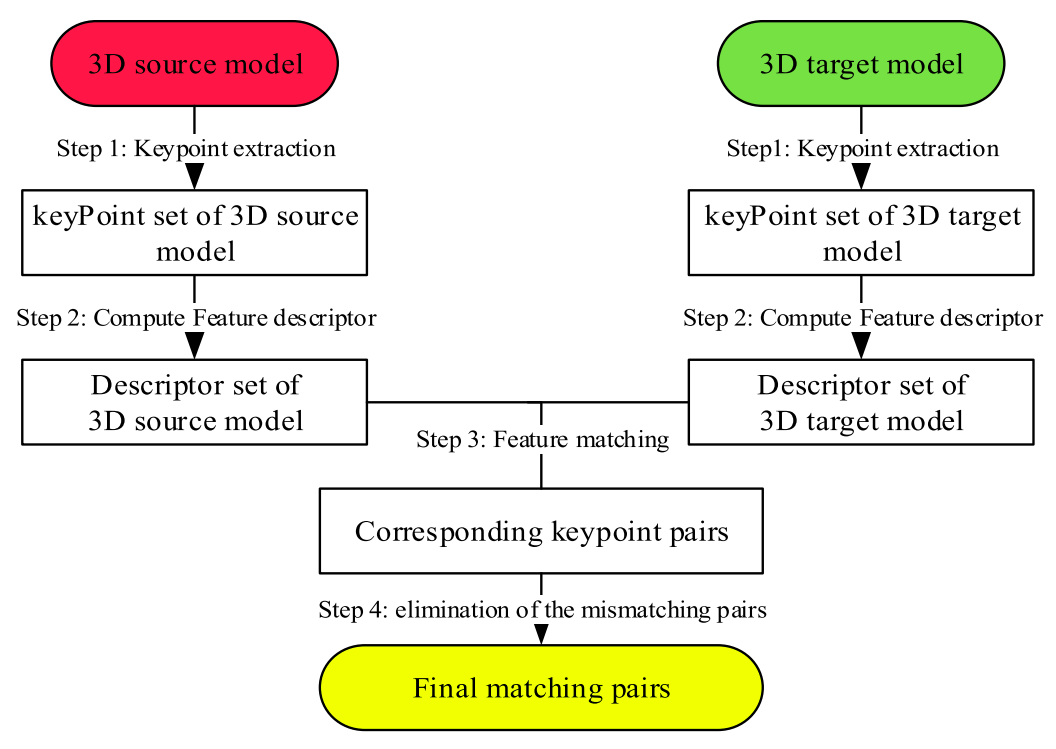
\includegraphics[scale=0.2]{images/covariance.png}
    \caption{\textit{Pipeline} de DGR}
    \label{fig:covariance}
\end{figure}

Este método es robusto, debido a que obtiene más del 70\% de \textit{accuracy} con 50\% de ruido, a comparación de otros métodos donde el \textit{accuracy} se degrada rápidamente a 30\% en promedio. Sin embargo, la experimentación se realizó únicamente sobre \textit{Puzzles 3D}, por lo cual no tenemos resultados sobre el \textit{accuracy} con fragmentos reales.

\section{\textit{Framework} probabilístico}

En el método de Wang \textit{et al.} la etapa de correspondencia está fusionada con la etapa de alineación. Por lo cual, el proceso se repite iterativamente hasta que el objeto está completamente reconstruido.\\

El método se compone de tres etapas principales. Primero, se detectan los bordes de los fragmentos con un algoritmo de crecimiento por región, donde se extraen los descriptores \textit{2D Link-Chain} (LCD) para cada borde. Segundo, se extrae el emparejamiento potencial con una estrategia de correspondencia deslizante entre descriptores, y se calcula el descriptor \textit{3D Spatial-Distribution} (SDD) para las áreas sobrepuestas. Tercero, se obtiene la similitud del emparejamiento potencial, y se realiza la detección de colisiones para eliminar los pares incorrectos \cite{7}. \\

Este método es versátil porque obtiene resultados notables con fragmentos de diferentes características. Sin embargo, en los casos extremos, como el reensamblaje de objetos con alta curvatura, el \textit{accuracy} disminuye significativamente. 
\end{comment}


\begin{comment}

\begin{itemize}
  %  \item \cite{2}. Dataset propio.
    \item \cite{3}. Puzzles 3D y dataset propio.
   % \item \cite{4}. Dataset propio.
    \item \cite{5}. Puzzles 3D y dataset propio (huesos).
    \item \cite{6}. Puzzles 3D.
    \item \cite{7}. Puzzles 3D, PRESIOUS y dataset propio (vasijas incluidas).
\end{itemize}

Una revisión de la literatura es un resumen crítico y analítico, y una síntesis del conocimiento actual de un tema. Una revisión de la literatura es mucho más que una lista de revisiones separadas de artículos y libros debe comparar y relacionar diferentes teorías, hallazgos, etc., en lugar de resumirlos individualmente. También debe tener un enfoque o tema particular para organizar la revisión.  Recuerde que no tiene por qué ser un relato exhaustivo de todo lo publicado sobre el tema, sino debería discutir toda la literatura académica más significativa e importante para ese enfoque.

El estado del arte o revisión bibliográfica permite pocisionar nuestro proyecto dentro de los trabajos ya existentes en la literatura científica. En la revisión bibliográfica se deben revisar solamente documentos pertenecientes a la literatura primaria y secundaria, evitando la literatura terciaria y gris y la literatura no científica. Es importante definir el formato de la citaciones (e.g., APA) y las forma correcta de hacerlo.

Existen varias técnicas para construir esta parte de un proyecto de investigación. Podemos utilizar una técnica poco formal, como la Revisión Empírica o Narrativa o podemos utilizar una técnica mas estructurada como la Revisión Sistemática~\cite{moreno2018revisiones}.

La revisión de la literatura debe concluir con un resumen y una pequeña discusión.

\end{comment}
